\section{The Muon System}
\label{sec:muon_sys}
Although it is the farthest system from the interaction point, the muon system is one of the most important subsystems within the Compact \emph{Muon} Solenoid experiment.
%  is the {\bf Muon System} and is what puts the {\it Muon} in Compact {\it Muon} Solenoid.
Of the particles emerging from the interaction point, electrons and photons are absorbed by the ECAL (Sec.~\ref{sec:ecal}) and hadronic matter is absorbed by the HCAL (Sec.~\ref{sec:hcal}).
This filtration process leaves only neutrinos and muons to enter the muon system, which is the outermost detector situated past the solenoid (Sec.~\ref{sec:solenoid}).
As mentioned in Ch.~\ref{ch:theory}, neutrinos are the only weakly interacting, electrically neutral SM particles which makes them incredibly difficult to detect directly.
In fact, neutrinos interact with normal matter so little that a light-year of lead (9.46 \emph{trillion}\Km) would only stop half of the neutrinos moving through it.
So, detection of neutrinos produced from \pp collisions is inferred via \MET on a per-event basis.
Muons, on the other hand, have a mass of 105.7\MeV (relatively heavy for a weakly-interacting, electrically-charged particle) and live approximately \tentothe{17} times longer than a Higgs boson: the average lifetime of a muon is $\tau_{\Pmu} = 2.2 \times \tentotheminus{6}\snd$.
% which interestingly will travel way outside of CMS before decaying, upwards of 100s of kilometers before decaying to an electron and neutrino (neutrinos are the only particles which CMS can't explicitly detect).
These properties are what determined the properties of the muon system within CMS to consist of its four main subdetectors, each of which is described in the following subsections:
\begin{enumerate}
    \item CSC (cathode strip chambers, Sec.~\ref{sec:csc}),
    \item DT (drift tubes, Sec.~\ref{sec:dt}),
    \item RPC (resistive plate chambers, Sec.~\ref{sec:rpc}),
    \item GEM (gas electron multiplier, Sec.~\ref{sec:gem}).
\end{enumerate}

\subsection{Cathode Strip Chambers}
\label{sec:csc} 

\textit{\textbf{Overview:}}
A cathode strip chamber (CSC) is a multi-wire proportional chamber capable of precisely measuring the position of muons which enter and ionize the gas within.
Spatial coordinates are obtained by the collection of electrical signals along the cathode strips $(\phi)$, anode wires $(r)$, and across multiple CSC layers $(z)$.
CSCs are found exclusively on the two endcaps of CMS---with each endcap bearing 270 chambers (Fig.~\ref{fig:cms_endcap})---so that there are 540 CSCs in total.
The chambers are arranged azimuthally around the beam pipe in four disks per endcap allowing for contiguous coverage in $\phi$.
In total, the CSC system provides an effective detection area of about 5000$\meter^2$, has a total gas volume that exceeds $> 50\meter^{3}$, and contains over 400\,000 read-out channels.
%%%%%%%%%%%%%%%%%%%%
\begin{multiFigure}
    \centering
        \addFigure{0.44}{figures/cms/muonsys/csc_endcap_cutaway.png}
        \addFigure{0.52}{figures/cms/muonsys/csc_endcap_real.png}
    \captionof{figure}
        [Cathode strip chambers line the disks of CMS]
        {Cathode strip chambers line the disks of CMS.
        \;A) Simulated cut-out view of the ME$+$ endcap, with the coordinate system of CMS on the left-hand side.
        Human for scale.
        \;B) The actual ME$-$2 disk of CMS is shown, revealing its ME$-$2/1 and ME$-$2/2 rings of CSCs.
        Figures taken from~\cite{collaboration_cms_2008}.}
    \label{fig:cms_endcap}
\end{multiFigure}
%%%%%%%%%%%%%%%%%%%%
% Longitudinal cross section
\begin{multiFigure}
    \centering
        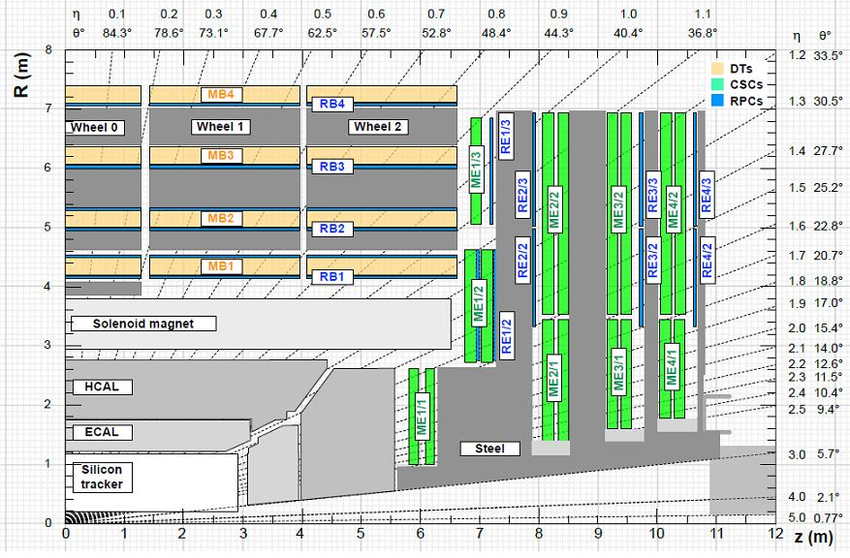
\includegraphics[width=15cm,height=10cm,keepaspectratio]{figures/cms/cms_longitudinal_view.png}
    \captionof{figure}
        [Longitudinal cross section of CMS with pseudorapidity values shown]
        {Longitudinal cross section of CMS showing the different pseudorapidity values ($\eta$), along with the different subdetector regions.
        Figure taken from~\cite{cms_long_xs_view}.}
    \label{fig:cms_long_view_subdetectors}
\end{multiFigure}
%%%%%%%%%%%%%%%%%%%%
\textit{\textbf{Design:}}
Each CSC is trapezoidal in shape with its narrow end pointed toward the beam pipe (Fig.~\ref{fig:csc_guts}).
The chambers are arranged in rings and each chamber subtends either 10\degrees or 20\degrees in $\phi$, as described in Sec.~\ref{sec:csc_numbering}.
The CSCs cover the pseudorapidity range of $0.9 < \abseta < 2.4$ (Fig.~\ref{fig:cms_long_view_subdetectors}).

A single CSC is composed of six layers (or \emph{gas gaps}), each of which is filled with a carefully prepared gaseous mixture\footnote{
    The gas mixture ratio of Ar:CO$_{2}$:CF$_{4}$ was chosen to be 5:4:1 to maximize the lifetime of the CSCs as they endure radiation damage through years of use.
    The CO$_{2}$ is used as a non-flammable quencher to reach even larger electron multiplicities, while the CF$_{4}$ helps prevent polymerization along (aging of) the wires.
    }
of Ar:CO$_{2}$:CF$_{4}$ (Fig.~\ref{fig:csc_separatelayers}).
Within every layer, the gas mixture surrounds approximately 80 copper strips, each of which spans radially away from the interaction point.
A single strip is about 8.4\mm wide at the narrower end of the CSC, about 16\mm at the wider end, and is separated from its neighboring strip by about 0.5\mm.
Per layer, the inner gas also surrounds over 1000 gold-plated tungsten wires, which are oriented azimuthally (so approximately orthogonal to the strips).
% (except in the CSCs closest to the interaction point)
Each wire is approximately 50\mum in diameter and separated from its neighboring wire by about 3.2\mm.
A collection of 16 consecutive wires forms a \emph{wire group}, which is about 5\cm wide and creates a single anode read-out channel.
A single wire plane has five independently controlled HV segments (Fig.~\ref{fig:csc_guts}).
The largest CSCs are 3.4\meter long as measured along a strip and 1.5\meter wide as measured along a wire.
% CSC separated layers.
%%%%%%%%%%%%%%%%%%%%
\begin{multiFigure}
    \centering
        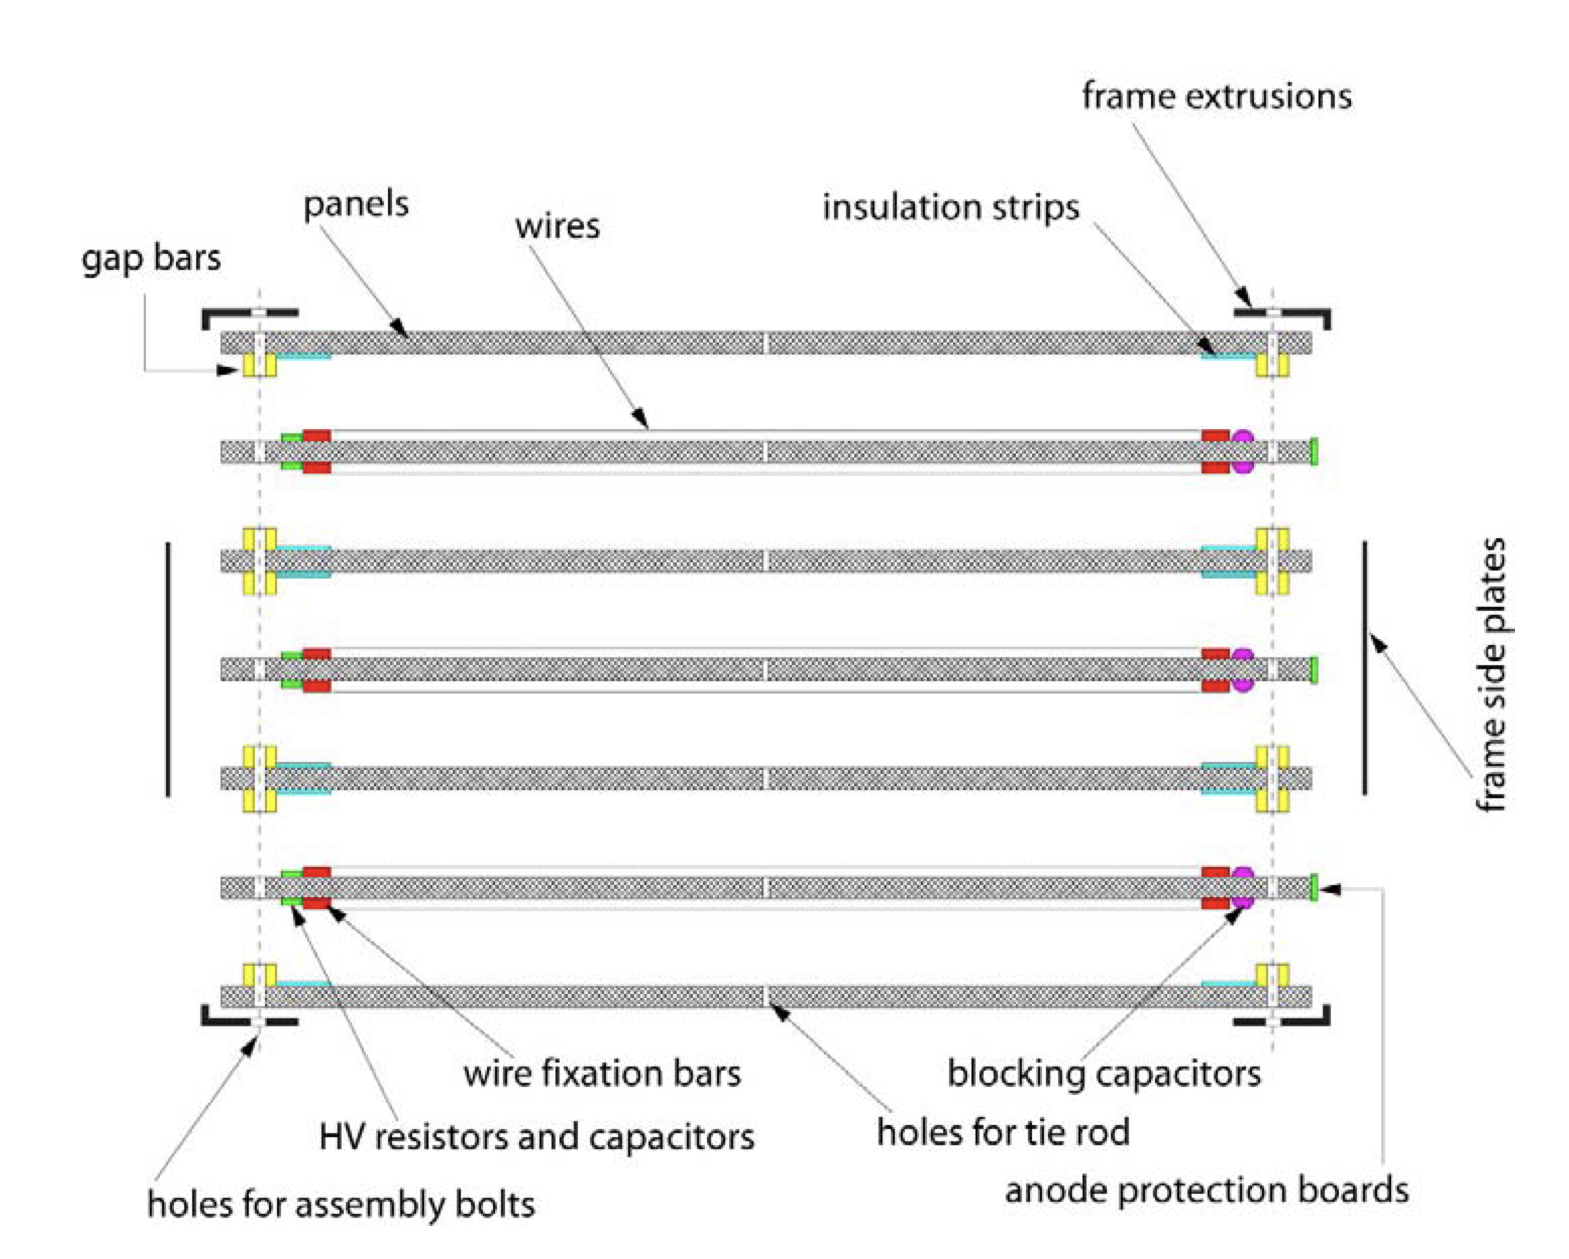
\includegraphics[width=0.9\textwidth,keepaspectratio]{figures/cms/muonsys/csc_separatedlayers.jpeg}
    \captionof{figure}
        [Cross section of CSC revealing the gas gaps]
        {Exploded view of the cross section of a CSC showing how the 7 panels come together to form the 6 gas gaps between the panels.
        Figure taken from~\cite{collaboration_cms_2008}.}
    \label{fig:csc_separatelayers}
\end{multiFigure}
% CSC guts.
%%%%%%%%%%%%%%%%%%%%
\begin{multiFigure}
    \centering
        \addFigure{0.41}{figures/cms/muonsys/csc_cutaway_view_new.png}
        \addFigure{0.55}{figures/cms/muonsys/csc_stripsandwires.png}
    \captionof{figure}
        [Views of an exposed CSC showing the wires and strips inside]
        {Views of an exposed CSC showing the wires and strips inside.
        \;A) CSC with its top layer exposed.
        Thin, horizontal, gold-plated tungsten wires span the entire width of the CSC. 
        Thicker, vertical strips run along the length.
        \;B) More detail inside a CSC showing the radial strips, horizontal wires, and 5 segments separating the wires.
        Figures taken from~\cite{collaboration_cms_2008}.}
    \label{fig:csc_guts}
\end{multiFigure}
% In conjunction with the Silicon Tracker measurements, muon momentum can be measured to a precision of 
% {\bf Quick Mention:} The University of Florida has been one of the main contributors to the CSC system and was home to one of the testing and assembly facilities before shipping the CSCs off to CERN.

\textit{\textbf{Physics:}}
As a muon passes through a CSC layer, it has the opportunity to interact with and ionize an Ar atom in the gas mixture.
The wires are under high voltage (3600\,V) which causes the ionized electron to accelerate towards the positively charged strips.
The accelerating electron collides with and ionizes Ar atoms along its path toward the strip.
This liberates even more electrons, thus forming an \emph{electron avalanche} (Fig.~\ref{fig:elec_avalanche}).
The total number of ionized electrons per initial electron is referred to as the \emph{multiplicity} (or \emph{gas gain}), which can reach as high as 100\,000.
% Electron avalanche.
%%%%%%%%%%%%%%%%%%%%
\begin{multiFigure}
    \centering
        \includegraphics[width=15cm,height=10cm,keepaspectratio]{figures/cms/muonsys/csc_elec_avalanche_old.png}
    \captionof{figure}
        [Muon traverses a CSC, ionizing the gas within and creating an electron avalanche]
        {A muon passes through one of the gaseous layers of the CSC, ionizing the gas mixture and inducing a charge on the anode wires and cathode strips.
        Figure taken from~\cite{collaboration_cms_2008}.}
    \label{fig:elec_avalanche}
\end{multiFigure}
%%%%%%%%%%%%%%%%%%%%

The electron avalanche is collected by a cathode strip and becomes an electrical signal.
This signal is processed by the cathode front-end boards (CFEBs).
The Ar$^+$ ions similarly distribute a charge signal onto the negative wires.
The cluster of charge that arrives at a strip is more widely spread than the charge which arrives along a wire.
Therefore, comparator logic is implemented on the strips to narrow down the precision to the order of 100\mum by using half-strip information (Fig.~\ref{fig:comparators}).
% Comparators and strips.
%%%%%%%%%%%%%%%%%%%%
\begin{multiFigure}
    \centering
        \addFigure{0.49}{figures/cms/muonsys/csc_comparator_logic.png}
        \addFigure{0.49}{figures/cms/muonsys/csc_comparator_logic_muontraverse.png}
    \captionof{figure}
        [Comparator logic as a muon traverses the layers of a CSC]
        {Comparator logic as a muon traverses the layers of a CSC.
        \;A) Comparators are used to compare neighboring strip cluster charge to determine on which half-strip the peak charge resided.
        \;B) Muon passes through all six layers of a CSC inducing charge on various half-strips.
        Figures taken from~\cite{collaboration_cms_2008}.}
    \label{fig:comparators}
\end{multiFigure}
%%%%%%%%%%%%%%%%%%%%

The muon passes through the next 5 layers of the CSC, further ionizing the gas mixture and generating electrical signals along the wires and strips.
A signal on a wire provides an $r$-coordinate, on a strip provides a $\phi$-coordinate, and through the other layers provides a $z$-coordinate.
Taken together, this information helps to reconstruct the three-dimensional trajectory of the muon.
% The AFEBs then digitize this analog signal using ADCs and 

The number of hits recorded by the CSC will determine if an event was significant enough to be worth saving.
If so, then its precise positions on the wires and strips will be read out by the Data Acquisition (DAQ) system and be stored for further data analysis.
When a CSC is taking live data it can resolve approximately 2\mm in $r$-$\phi$, whereas during offline analysis the resolution improves by a factor of more than 20:
the ME1/1 and ME1/2 chambers can resolve distances as small as 75\mum in $r$-$\phi$, while the other chambers can resolve 150\mum.
It is worth noting that a CSC can accommodate up to 1$\KHz/\cmns^2$.

% Each CSC cost about \$100,000 to make, so very quickly this becomes an expensive project.

% Gas gap is 9.5~\mm.

% \subsection{Endcap Muon Electronics}
% In order to conclude that a muon definitely passed by the muon detectors, a very sophisticated electronics system has been developed. 

% Hmm... EMU is just for the endcaps. This system is called "EMU" and 

% Next I am going to elaborate more on the CSCs, since my first experience with CMS hands-on work with CSCs. 

% The muon barrel system, after it talks with the tracker system, has a muon pT resolution of 1.5% in the barrel and ~6% in the endcap.

% Trigger system:
% Since the event  rate and data rate are so high, and most of the events are uninteresting, typical physics,
% we need a fast-working filtration system to sift through the good and bad events. 
% We want to "trigger" on the good events but only have about 4 μs to do so. 
% This is the job of the L1 trigger and and the High-Level Trigger. 

\subsubsection{CSC Numbering Scheme}
\label{sec:csc_numbering}
The two endcaps are labelled as `ME$+$' and `ME$-$', depending on whether they are situated in the $+z$ direction or $-z$.
Both endcaps are structurally symmetric, so it is sufficient to discuss only one in detail.
The ME$+$ endcap has four disks: ME$+$1 is the first disk and the one closest to the interaction point, while ME$+$4 is the fourth and the farthest away. 
Within each disk, there are either two or three \emph{rings} of CSCs, as shown in Fig.~\ref{fig:cms_long_view_subdetectors} (green).
These rings are labelled as ME$+D$/$R$, where $D$ indicates the disk number and $R$ indicates the ring number.
For example, ME$+$2/1 refers to the second disk and the first ring (the ring closest to the beam pipe).
All rings contain 36 CSCs, except for ME$\pm X$/1, for $X= 2,3,4$, which contain only 18 CSCs.
Finally, the CSCs are given one final number to label them on the ring:
the CSC that sits along the positive $x$ axis in the coordinate system of CMS is given the number `01', \eg ME$+$4/2/01. 
The CSCs are then numbered incrementally following the positive azimuthal direction.

\subsection{Drift-Tube Chambers}
\label{sec:dt}

\textbf{\textit{Overview:}}
Functionally similar to but structurally different from a CSC (Sec.~\ref{sec:csc}), a DT is a collection of gaseous detector cells (Fig.~\ref{fig:dt_superlayers}).
A single DT cell has an anode wire and two cathode strips and operates on the same principle as a CSC, providing timing and position measurements of muons (Fig.~\ref{fig:dt_cell}).
While CSCs are found only on the endcaps of CMS, drift-tube chambers (DTs) are placed exclusively along the barrel (Fig.~\ref{fig:dt_locations}).
The DT system is therefore composed of concentric cylindrical stations, with the central axis parallel to the beam pipe.
Altogether, there are 250 DTs built inside of, between, and outside of the iron yoke.
% DT Chamber.
%%%%%%%%%%%%%%%%%%%%
\begin{multiFigure}
    \centering
        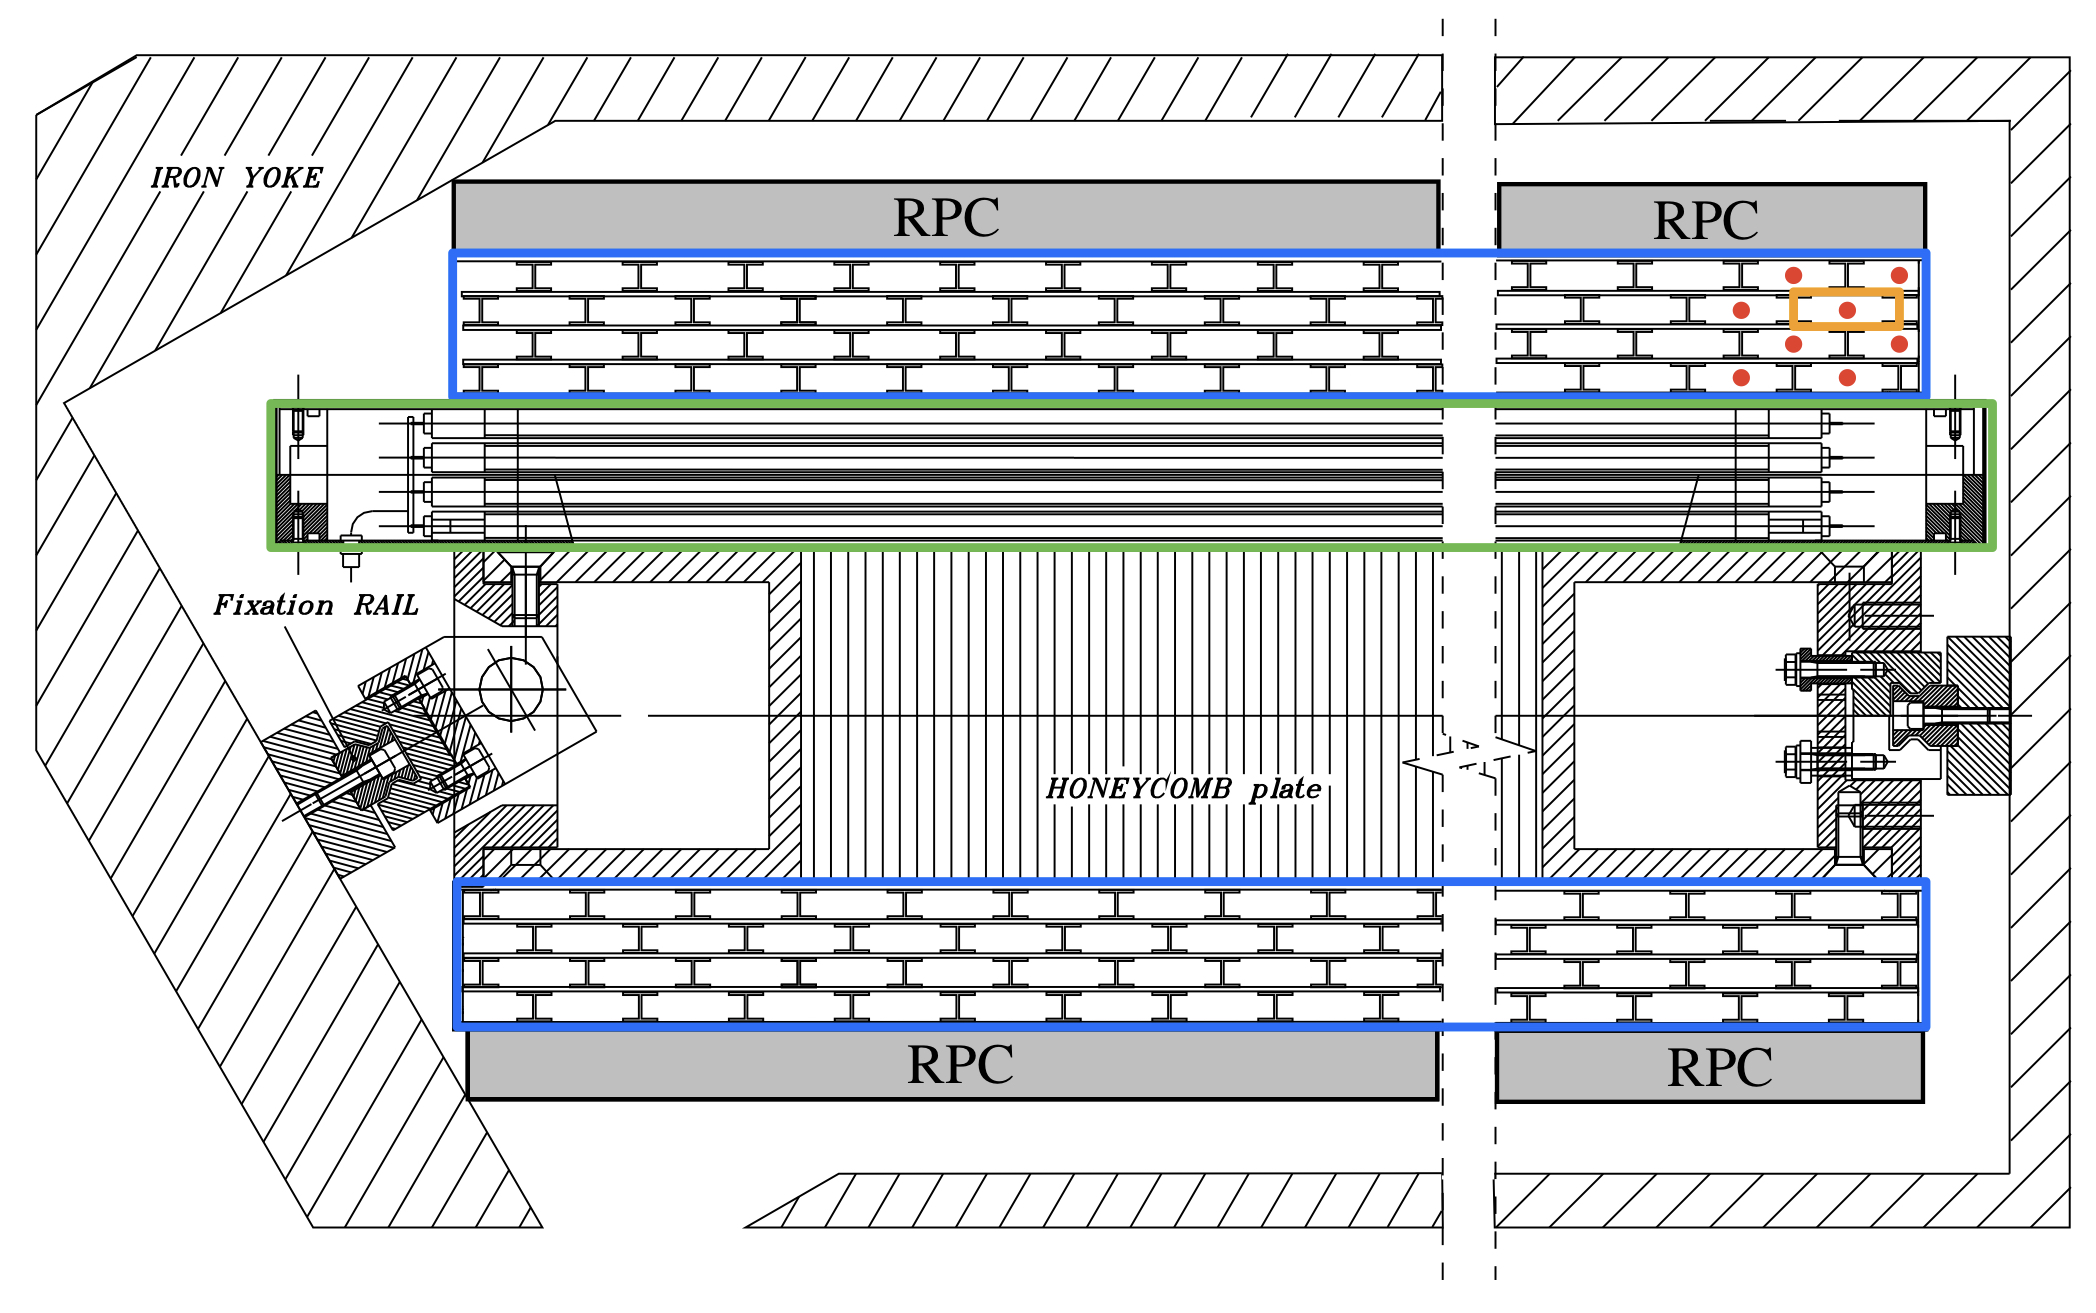
\includegraphics[height=9cm,keepaspectratio]{figures/cms/muonsys/drifttube_superlayers.jpeg}
    \captionof{figure}
        [Cross section of an entire drift tube chamber]
        {Cross section of an entire drift tube (DT) chamber showing 3 superlayers (SLs) and the interior honeycomb plate.
        Two SLs are indicated by the blue rectangles, whose cells (orange rectangle) have anode wires (red dots) oriented parallel to the beam pipe.
        The third SL is indicated by the green rectangle and is placed orthogonally to the other two SLs.
        Figure taken from~\cite{collaboration_cms_2008} and modified with orange, green, and blue rectangles and red dots.}
    \label{fig:dt_superlayers}
\end{multiFigure}
% DT Cell.
%%%%%%%%%%%%%%%%%%%%
\begin{multiFigure}
    \centering
        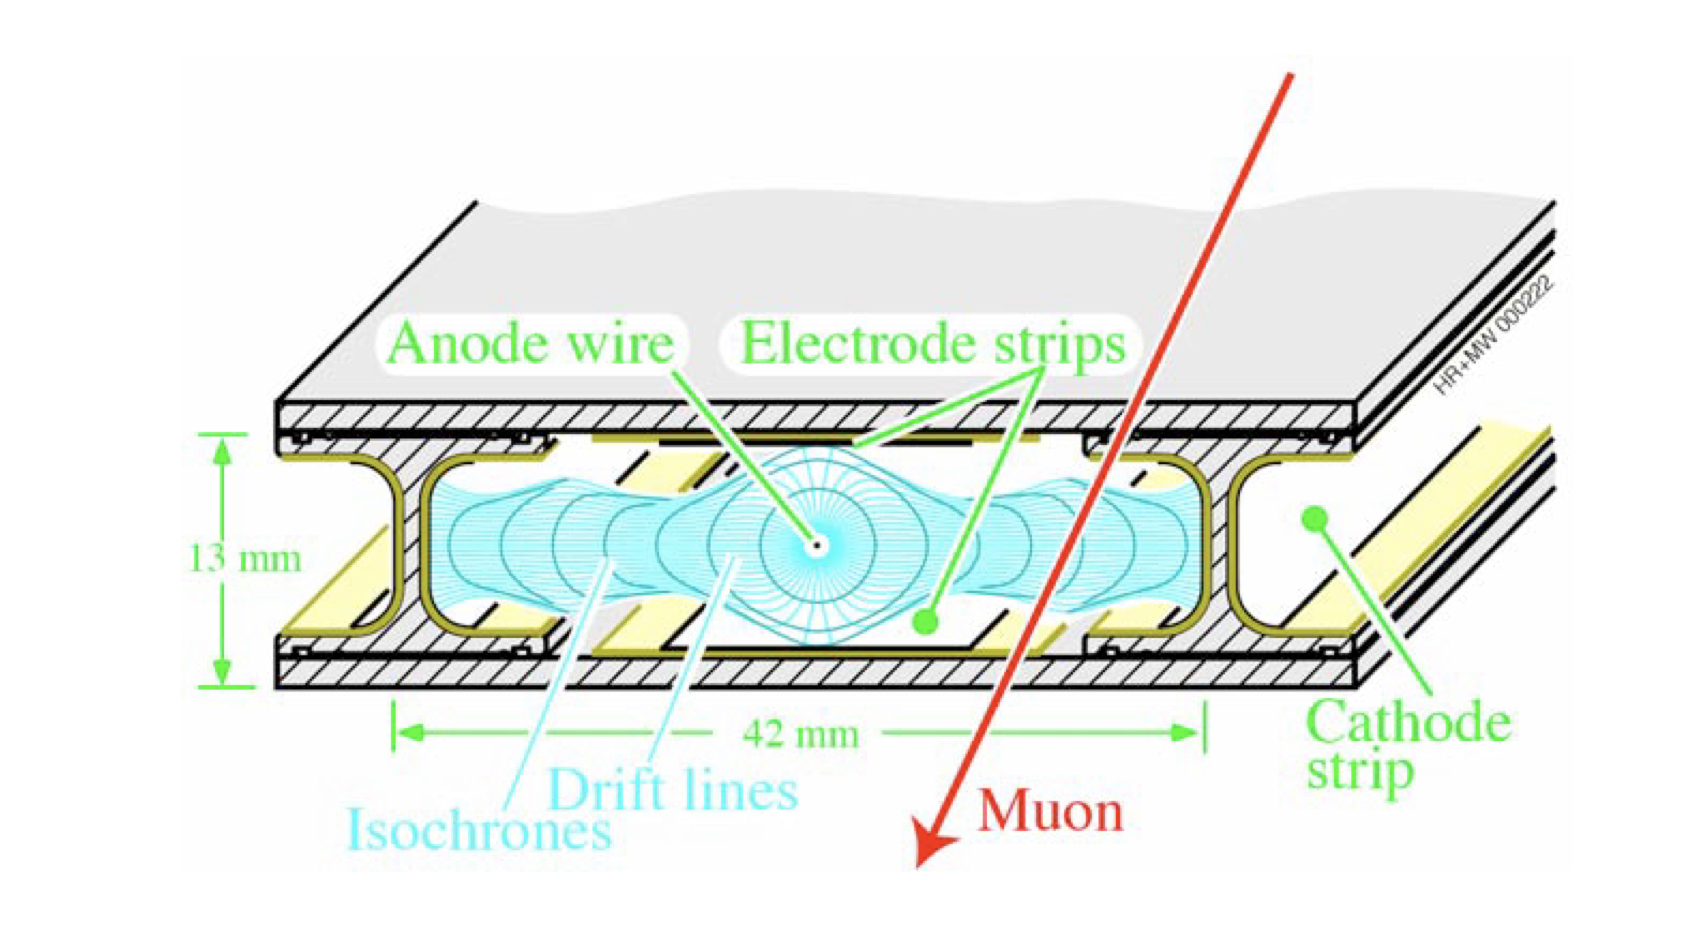
\includegraphics[height=5.5cm,keepaspectratio]{figures/cms/muonsys/drifttube_xs.jpeg}
    \captionof{figure}
        [Cross section of a single drift tube cell]
        {Cross section of a single drift tube cell showing the drift lines (light blue), isochrone lines (dark blue), dimensions of the cell, and locations of the anode wire and cathode strips.
        Figure taken from~\cite{collaboration_cms_2008}.}
    \label{fig:dt_cell}
\end{multiFigure}
%%%%%%%%%%%%%%%%%%%%
% DT locations.
\begin{multiFigure}
    \centering
        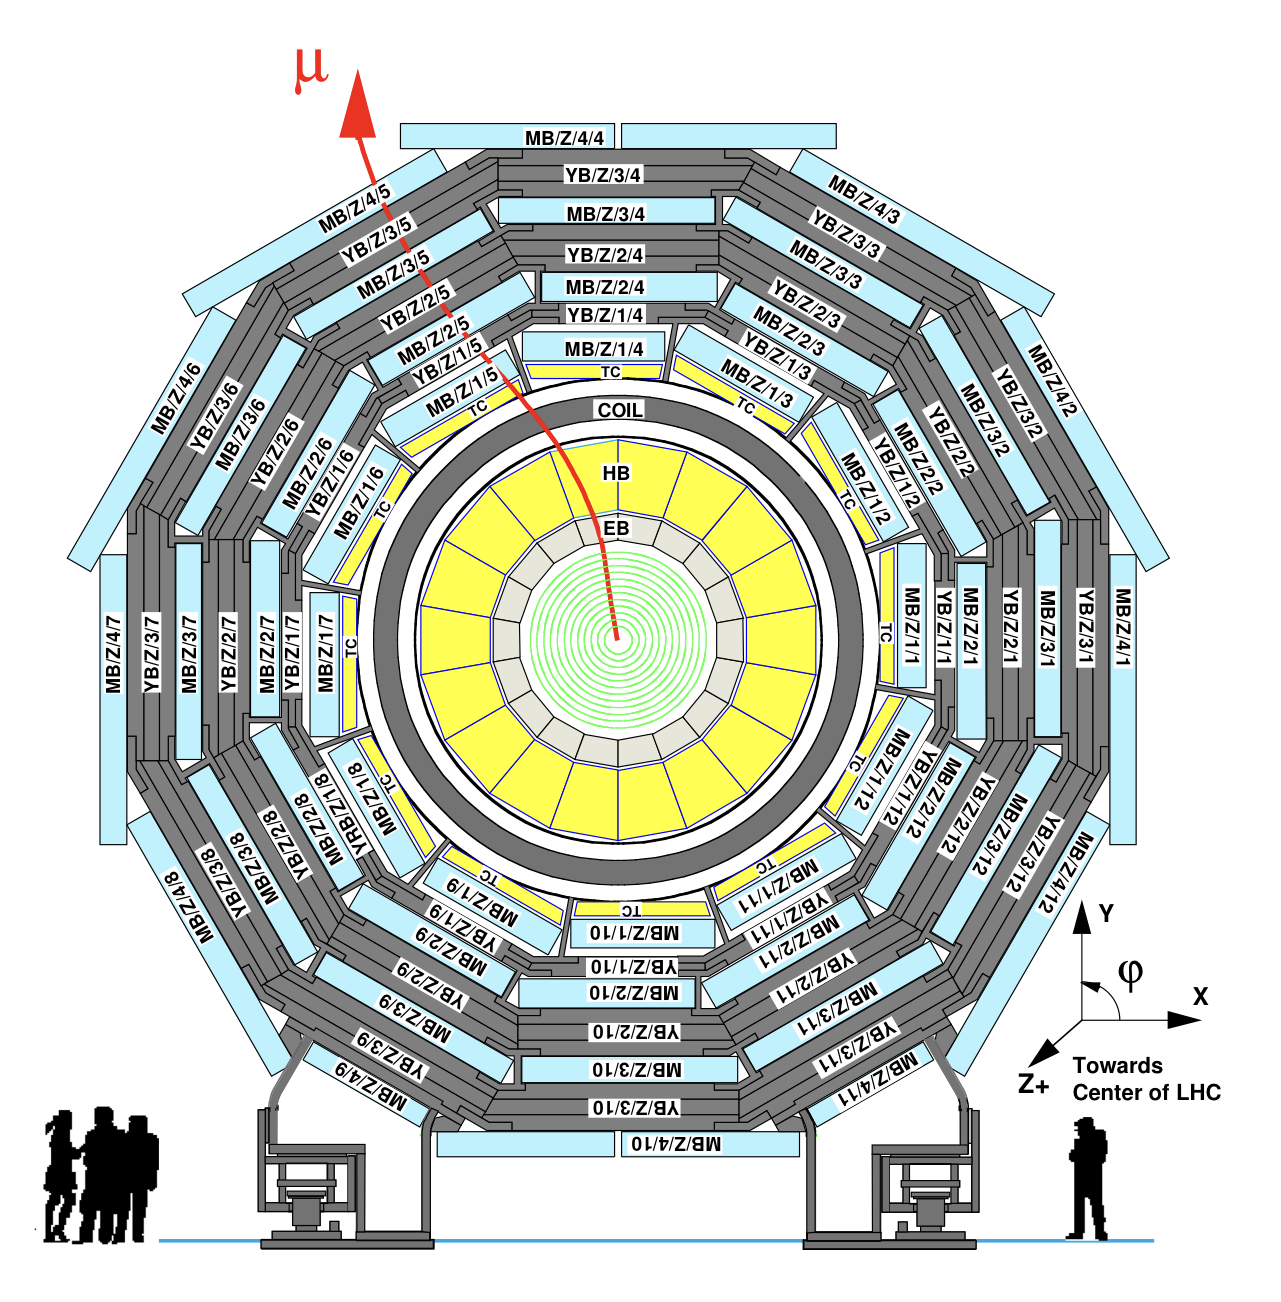
\includegraphics[width=15cm,height=10cm,keepaspectratio]{figures/cms/muonsys/drifttube_locations.jpeg}
    \captionof{figure}
        [Cross section of the CMS barrel showing the locations of the drift tubes]
        {Cross section of the CMS barrel showing the locations and the numbering scheme of the drift tubes in the barrel.
        Figure taken from~\cite{collaboration_cms_2008}.}
    \label{fig:dt_locations}
\end{multiFigure}
%%%%%%%%%%%%%%%%%%%%

\textbf{\textit{Design:}}
The first three stations contain 60 DTs each, while the station farthest from the beam pipe contains 70 DTs.
The DTs are distributed among 5 wheels, 4 stations, and 12 sectors within the muon barrel (MB) system which uses the following numbering scheme:
MB/$W$/$A$/$S$,
where $W$ is the wheel number ($-$2 to 2),
$A$ is the station number (1 to 4),
and $S$ is the sector number (1 to 12).
This accounts for only $5 \times 4 \times 12 = 240$ chambers, so the remaining 10 DTs are found in station 4, sectors 4 and 10, in each wheel (Fig.~\ref{fig:dt_locations}).

Each tube cross section is $13 \times 42\mm^{2}$, within which a single anode wire is made of gold-plated stainless-steel that has a diameter of 50\mum.
Different voltages are applied to the anode wires ($+$3600\,V), electrode strips ($+$1800\,V), and cathode strips ($-$1200\,V).
The gas mixture within a DT is similar to that of a CSC, containing approximately 85\% Ar $+$ 15\% CO$_{2}$.

\textbf{\textit{Physics:}}
DTs are a good choice for the barrel because of the low rate and low strength of magnetic field.
They offer a uniform drift field of 1.5\,KV/cm.
A high \pt muon track will cross all 4 DT stations within the pseudorapidity range of $\abseta < 0.8$.
The reconstruction efficiency of such a track is better than 95\%.

A single SL has a time resolution of only a few nanoseconds which provides excellent bunch crossing identification.
To assist in determining muon \pt and timing, the DT system delivers the following muon track segment information to the L1 trigger:
the position of the center of gravity (to a precision of 1.5\mm) and the corresponding angle (to a precision of 20\,mrad), with respect to the SL reference frame.
The total resolution of a DT in the $r$-$\phi$ plane is about 100\mum which is comparable to the deviation caused by multiple scattering, for a muon with $\pt \le 200\GeV$.

The gas gain is comparable to that of a CSC (about 100\,000).
The maximum drift distance in a DT is 21\mm, as can be seen in Fig.~\ref{fig:dt_cell}, which corresponds to a drift time of 380~\ns.

\subsection{Resistive Plate Chambers}
\label{sec:rpc}

\textbf{\textit{Overview:}}
Even though CSCs (Sec.~\ref{sec:csc}) and (Sec.DTs~\ref{sec:dt}) cover the entire pseudorapidity range of $0 < \abseta < 2.4$, redundancy is important.
Therefore, resistive plate chambers (RPCs) are placed in both the barrel and endcaps to provide excellent timing and spatial resolution---comparable to that of scintillators---to supplement the measurements of the CSC and DT systems.
RPCs are fast, gaseous detectors that serve as a muon trigger system.
Muons traversing through the RPCs ionize the gas and cause an avalanche, which is measured by the plate.

\textbf{\textit{Design:}}
% RPCs consist of two highly-resistive parallel plates (bakelite electrodes), one positively-charged and the other negatively-charged, separated by a 2-\mmns gap of gaseous volume.
The gas is a three-component mixture composed of 95.2\% C$_2$H$_2$F$_4$, 4.5\% $i$C$_4$HO (isobutane), and 0.4\% SF$_6$ with a 35--40\% humidity, and kept at 21$\degrees$C.
The RPC system consists of 480 rectangular chambers found in the barrel and are oriented parallel to the beam pipe, each at 2.455\meter long.
There are also 288 RPCs found on each endcap.
RPCs have better time resolution compared to the 25\ns between two consecutive \pp bunch crossings. 

% Gas mixture comprised of 96.2\% C$_{2}$H$_{2}$F$_{4}$ (1,1,1,2-tetrafluoroethane) $+$ 3.5\% $i$C$_{4}$H$_10$ (isobutane) $+$ 

\textbf{\textit{Physics:}}
Muons passing through RPC chambers ionize the gas, causing an avalanche of electrons.
The electrodes are transparent to the signal, which are instead picked up by the external metallic strips after a small but precise time delay.
The pattern of strips which are hit gives a rapid measure of the muon's momentum, which is then used by the trigger to make an immediate decisiosn about whether the data are worth keeping.
RPCs combine a good spatial resolution with an excellent time resolution of just one nanosecond. 

\subsection{Gas Electron Multipliers}
\label{sec:gem}

\textbf{\textit{Overview:}}
Gas Electron Multipliers (GEM) are a new addition to the CMS muon system and will complement existing detectors in the forward regions close to the beampipe where radiation levels and event rates will significantly increase during Phase-2 of the LHC.
GEM systems in the endcaps will improve the measurement of the polar muon bending angle, allowing the muon trigger to cope with higher rates.
The GEMs will further extend the muon system coverage in the far-forward regions. 

\textbf{\textit{Design:}}
GEMs are gaseous detectors featuring a GEM foil, which consists of a 50-\mumns-thick insulating polymer (polyimide) encased on top and bottom by copper conductors.
Microscopic holes are etched in a regular hexagonal pattern throughout the foil.
The GEM chambers consist of two PCBs containing the gas volume filled with an Ar/CO$_2$ gas mixture separated by a stack of three GEM foils.
The GEMs feature a large area of about 0.5$\meter^2$.
The first batch comprising 144 chambers was installed during Long Shutdown 2 on the first disk of the two endcaps.
These chambers will contribute to data-taking during Run 3 of the LHC.
Additionally, two more disks of GEM chambers will be installed in each endcap during 2024--2026, before the Phase-2 upgrade.

\textbf{\textit{Physics:}}
The chambers are filled with an Ar/CO$_2$ gas mixture, which is ionized by muons traversing the detector system.
This generates a potential difference across the foils, which generates sharp electric fields in the holes.
Electrons created during the ionization process drift towards the foil and are multiplied in the holes, resulting in an electron avalanche that induces a readout signal on finely-spaced strips.





% We can only assume that we produced neutrinos when momentum is apparently not conserved in an event. 
% When the protons collide at the IP they have nearly zero momentum perpendicular to the beam pipe. 
% This is called transverse momentum, because it's well... transverse to the beam pipe, the z direction.
% If we track, tag, capture all the outgoing particles and reconstruct their transverse momenta, 
% if we find out that it is NOT zero by a large amount, then we say that 

% The main purpose of the Muon System is to precisely determine the position and timing of muons.
% \begin{enumerate}
%     \item 
%     % for offline analysis.
%     \item Generate muon trigger primitives for the Level-1 trigger system.
% \end{enumerate}
% Similar to the Silicon Tracker, the Muon System doesn't try to capture the muons passing through it;
% instead it just tracks their positions. 
% In fact our very own Andrey, Guenakh, and Darin have been instrumental in implementing CSCs. 
% There's also an assembly hall downstairs where CSCs were constructed and tested 
% The  specializes muons. Au contraire; it \textit{specializes} in muon detection. 
% The Compact \textit{Muon} Solenoid would be a pretty hypocritical name if CMS did not detect muons. Au contraire; it \textit{specializes} in muon detection. 
% P
%It would be an ironic name if it did not detect muons well. 

% This concludes the overall design and purpose of the subdetectors that make up CMS.
% Since I have had hands-on experience working on CSCs, I will discuss the CSC components and how it works in more detail in the subsection below.
